\documentclass{standalone}

\usepackage{tikz}
\usetikzlibrary{automata, positioning, arrows}
\tikzset{
	->,
	>=stealth,
	node distance=3cm,
	every state/.style={thick, fill=gray!10},
	initial text=$ $,
}

\begin{document}
	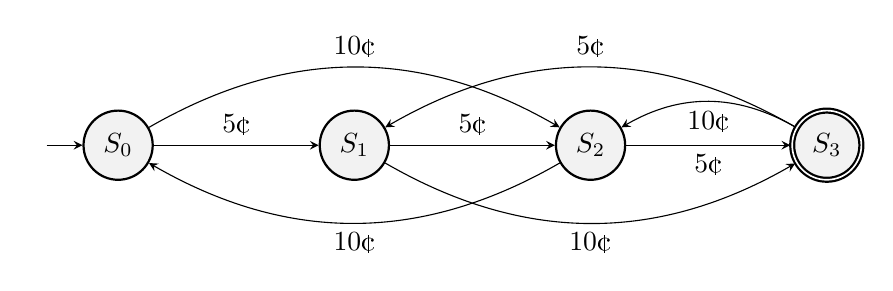
\begin{tikzpicture}
		\node[state, initial] (s0) {$S_0$};
		\node[state, right of=s0] (s1) {$S_1$};
		\node[state, right of=s1] (s2) {$S_2$};
		\node[state, accepting, right of=s2] (s3) {$S_3$};
		\draw (s0) edge[above] node{5\textcent} (s1)
			(s0) edge[bend left, above] node{10\textcent} (s2)
			(s1) edge[above] node{5\textcent} (s2)
			(s1) edge[bend right, below] node {10\textcent} (s3)
			(s2) edge[below] node {5\textcent} (s3)
			(s2) edge[bend left, below] node {10\textcent} (s0)
			(s3) edge[bend right,below] node {10\textcent} (s2)
			(s3) edge[bend right, above] node {5\textcent} (s1);
	\end{tikzpicture}
\end{document}